\documentclass{article}
\usepackage[utf8]{inputenc}
\usepackage{amsmath}
\usepackage{amsthm}
\usepackage{bm}
\usepackage{wrapfig}
\usepackage{graphicx}
\usepackage{ mathrsfs }
\usepackage[a4paper, total={6in, 8in}]{geometry}

\graphicspath{ {extras/} }

% per usare la r corsiva di griffiths
% punti esclamativi per togliere lo spazio extra strano
\def\rcurs{{\mbox{$\resizebox{.16in}{.08in}{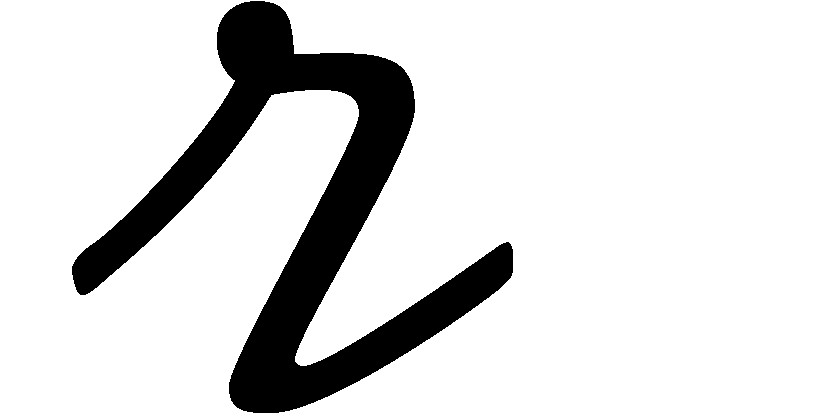
\includegraphics{ScriptR}}$}} \!\!}
\def\brcurs{{\mbox{$\resizebox{.16in}{.08in}{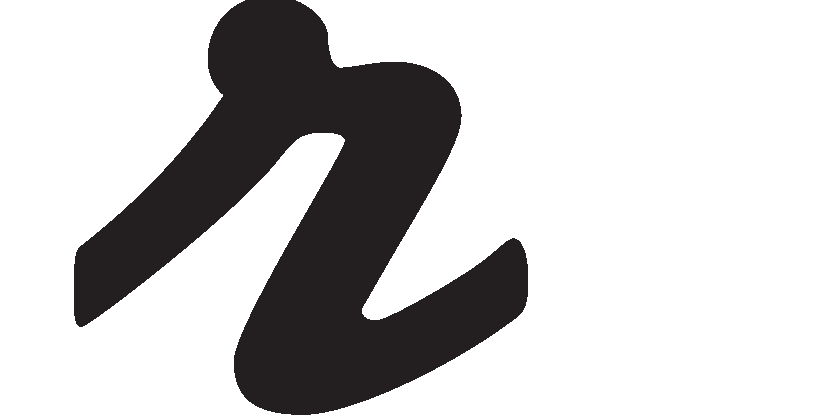
\includegraphics{BoldR}}$}}}
\def\hrcurs{{\mbox{$\hat \brcurs$}} } 

\renewcommand{\epsilon}{\varepsilon}
\newcommand{\ez}{\epsilon_0}
\newcommand{\mbf}{\mathbf}
\newcommand{\vers}[1]{\mbf{\hat #1 }}
\newcommand{\qpe}[1][1]{ \frac{ #1 }{ 4\pi\epsilon_0 } }
\newcommand{\rot}[1][]{\nabla#1 \times}  % il parametro è in caso voglia mettere l'apostrofo per derivare rispetto a coord primate
\newcommand{\grad}[1][]{\nabla#1}
\renewcommand{\div}[1][]{\nabla#1 \cdot}

\numberwithin{equation}{section}

\title{ Electromagnetism }
\author{William Luciani}
\date{July 2021}

\begin{document}

\maketitle

\tableofcontents

\pagebreak


\section{Costanti} % (fold)
\label{sec:costanti}

\begin{align}
    \epsilon_0  &= 8.85     \cdot 10^{-12}  \; \mathrm{ C^2 / N m^2 }\\
    e           &= 1.6      \cdot 10^{-19}  \; \mathrm{ C }\\
\end{align}

% section costanti (end)

\section{Strumenti matematici} % (fold)
\label{sec:strumenti_matematici}

\subsection{Vettori} % (fold)
\label{sub:vettori}

Prodotto misto: 

\begin{equation}
    \mbf{ A \cdot ( B \times C ) }
\end{equation}
è possibile ciclare i tre vettori
\begin{equation}
    \mbf{ A \cdot ( B \times C ) } =
    \mbf{ B \cdot ( C \times A ) } =
    \mbf{ C \cdot ( A \times B ) }
\end{equation}
e anche scambiare prodotto scalare e vettoriale
\begin{equation}
    \mbf{ A \cdot ( B \times C ) } = \mbf{ ( A \times B ) \cdot C }
\end{equation}

Doppio prodotto vettore. Vale la regola del BAC-CAB:

\begin{equation}
    \mbf{ A \times ( B \times C ) } = \mbf{ B ( A \cdot C) - C ( A \cdot B) }
\end{equation}
Non è associativo ma vale l'identità di Jacobi:
\begin{equation}
    \mbf{ A \times ( B \times C ) } +
    \mbf{ B \times ( C \times A ) } +
    \mbf{ C \times ( A \times B ) } = 0
\end{equation}

% subsection vettori (end)

\subsection{Analisi Vettoriale} % (fold)
\label{sub:analisi_vettoriale}



Derivazione in coordinate cartesiane. Operatore nabla:
\begin{equation}
    \nabla = \partial_x \vers x + \partial_y \vers y + \partial_z \vers z
\end{equation}

Gradiente: 
\begin{equation}
    \nabla f = \partial_x f \vers x + \partial_y f \vers y + \partial_z f \vers z
\end{equation}

Rotore: 
\begin{equation}
    \nabla \times \mbf A = 
    \begin{vmatrix}
        \vers i     & \vers j       & \vers k       \\
        \partial_x  & \partial_y    & \partial_z    \\
        A_x         & A_y           & A_z
    \end{vmatrix}
\end{equation}

Divergenza: 
\begin{equation}
    \nabla \cdot \mbf A = \partial_x A_x + \partial_y A_y + \partial_z A_z
\end{equation}


\subsubsection{Gradiente} % (fold)
\label{ssub:gradiente}


Il gradiente può anche essere definito nel seguente modo, indipendente dalle coordinate usate.
\begin{equation} \label{eq:grad_def}
    ( \nabla f ) \cdot \vers t = \lim_{ dl \to 0 }  \frac{ df }{ dl } 
\end{equation}
Dove la variazione di f è presa lungo un tratto infinitesimo di lunghezza $dl$ e direzione $\vers t$.

Passando ad un percorso finito $\gamma$ si ha 
\begin{equation*}
    \int_\gamma ( \nabla f ) \cdot \vers t dl = \Delta f
\end{equation*}

Questo è il teorema del gradiente (o teorema fondamentale del calcolo), che può esser scritto anche nel seguente modo.
\begin{equation}
    \int_A^B \nabla f \cdot d \mbf l = f(B) - f(A)
\end{equation}

Per il gradiente c'è un modo più immediato di trovare la relazione sopra, ma il modo sopra è utile poichè è del tutto analogo al procedimento per il rotore e la divergenza.

Il modo più diretto è il seguente. Il differenziale di un campo vettoriale scalare può esser scritto nel seguente modo:
\begin{equation}
    df = \nabla f \cdot d \mbf l
\end{equation}
Integrando segue direttamente il teorema del gradiente.

% subsubsection gradiente (end)

\subsubsection{Rotore} % (fold)
\label{ssub:rotore}

Per il rotore vale la seguente definizione:
\begin{equation} \label{eq:rot_def}
    ( \nabla \times \mbf A ) \cdot \vers n 
        = \lim_{ dS \to 0 } \frac{ 1 }{ dS }  \int_\gamma \mbf A \cdot d \mbf l 
        = \lim_{ dS \to 0 } \frac{ dC }{ dS }
\end{equation}
Dove $dS$ è un'area infinitesima e $\vers n$ è la sua normale. $\gamma$ è il bordo di S, ovvero un circuito infinitesimo. $dC$ è la circuitazione attraverso questo circuito infinitesimo.

Passando ad una superficie $S$ finita si ha quindi:
\begin{equation*}
    \int_S ( \nabla \times \mbf A ) \cdot \vers n dS = C
\end{equation*}
Questo è il teorema di Stokes (o del rotore), che può esser scritto anche nel seguente modo. ($\partial S$ è il bordo di $S$)
\begin{equation}
    \int_S ( \nabla \times \mbf A ) \cdot d \mbf S = \int_{\partial S} \mbf A \cdot d \mbf l
\end{equation}


% subsubsection rotore (end)

\subsubsection{Divergenza} % (fold)
\label{ssub:divergenza}


Per la divergenza vale la seguente definizione:
\begin{equation}    \label{eq:div_def} 
    \nabla \cdot \mbf A 
        = \lim_{ dV \to 0 } \frac{ 1 }{ dV } \int_S \mbf A \cdot d \mbf S 
        = \lim_{ dV \to 0 } \frac{ d\Phi }{ dV }
\end{equation}
Dove $dV$ è un volume infinitesimo, $S$ è la sua superficie. $d\Phi$ è il flusso attraverso $S$.

Passando ad un volume finito si ha:
\begin{equation*}
    \int_V \nabla \cdot \mbf A dV = \Phi
\end{equation*}
Questo è il teorema della divergenza (o di Gauss), che può esser scritto anche nel seguente modo. ($\partial V$ è il bordo di $V$)
\begin{equation}
    \int_V \nabla \cdot \mbf A dV = \int_{\partial V} \mbf A \cdot d \mbf S
\end{equation}


% subsubsection divergenza (end)

\subsection{Derivate seconde} % (fold)
\label{sub:derivate_seconde}

Si possono fare le seguenti derivate seconde con l'operatore nabla:
\begin{enumerate}
    \item $\nabla \times \nabla f = 0 $ 
    \item $\nabla \cdot \nabla f =: \nabla^2 f = \Delta f$ Definizione del Laplaciano
    \item $\nabla \times \nabla \times A$ 
    \item $\nabla \cdot \nabla \times A = 0$ 
    \item $\nabla (\nabla \cdot A)$ 
\end{enumerate}
La 5. non è di particolare interesse e per la 3 vale la seguente uguaglianza:
\begin{equation}
    \nabla \times \nabla \times A = \nabla (\nabla \cdot A) - \nabla^2 A
\end{equation}
Per chiarezza esplicitiamo il laplaciano di un campo scalare e di un campo vettoriale:
\begin{align}
    \nabla^2 f &= \partial_x^2 f + \partial_y^2 f + \partial_z^2 f \\
    \nabla^2 A &= \nabla^2 A_x \vers x + \nabla^2 A_y \vers y + \nabla^2 A_z \vers z
\end{align}

% subsection derivate_seconde (end)

\section{Derivate di prodotti} % (fold)
\label{sec:derivate_di_prodotti}

Ci sono sei regole per le derivate di prodotti di funzioni. Due per il gradiente:
\begin{equation} \label{eq:grad_prod} 
    \grad (fg) = f \grad g + f \grad g                             
\end{equation}
\begin{equation} \label{eq:grad_prod_scal}
    \grad (\mbf A \cdot \mbf B) = \mbf A \times (\rot \mbf B) + \mbf B \times (\rot \mbf A)
                       + (\mbf A \cdot \nabla) \mbf B + (\mbf B \cdot \nabla) \mbf A    
\end{equation}
due per la divergenza:
\begin{equation} \label{eq:div_prod} 
    \div (f\mbf A) = f (\div \mbf A) + \mbf A \cdot (\grad f)
\end{equation}
\begin{equation} \label{eq:div_prod_vett} 
    \div (\mbf A \times \mbf B) = \mbf B \cdot (\rot \mbf A) - \mbf A \cdot ( \rot \mbf B)
\end{equation}
e due per il rotore:
\begin{equation} \label{eq:rot_prod} 
    \rot (f\mbf A) = f (\rot \mbf A) + (\grad f) \times \mbf A
\end{equation}
\begin{equation} \label{eq:rot_prod_vett} 
    \rot (\mbf A \times \mbf B) = (\mbf B \cdot \nabla) \mbf A - (\mbf A \cdot \nabla) \mbf B + \mbf A (\div \mbf B) - \mbf B(\div \mbf A)
\end{equation}

% section derivate_di_prodotti (end)


\subsection{Derivate utili} % (fold)
\label{sub:derivate_utili}

\begin{align} 
    \nabla \cdot \frac{ \vers r }{ r^2 } &= 4 \pi \delta(\mbf r)        \label{eq:derivate_utili_divr2} \\ 
    \nabla \cdot (r^n \vers r)  &= (n+2)r^{n-1}, \qquad n \neq -2       \label{eq:derivate_utili_div}   \\
    \nabla r^n &= n r^{n-1} \vers r                                     \label{eq:derivate_utili_grad}  \\
    \nabla \times (r^n \vers r) &= 0                                    \label{eq:derivate_utili_rot}   \\
\end{align}
Le stesse formule valgono anche sostituendo $\rcurs$ al posto di $r$. Nel caso di $\rcurs$ è possibile anche derivare rispetto alle coordinate primate, in quel caso compare un $-$.

% subsection derivate_utili (end)

% subsection analisi_vettoriale (end)

% section strumenti_matematici (end)



\section{Elettrostatica nel vuoto} % (fold)
\label{sec:elettrostatica_nel_vuoto}

\subsection{Formule Sperimentali} % (fold)
\label{sub:formule_sperimentali}

\begin{equation}
    \brcurs = \mbf r - \mbf r'
\end{equation}
Dove r è il punto in cui vogliamo calcolare il campo e r' è la posizione della carica. (Se pensiamo alla forza, r è la posizione della carica su cui calcoliamo la forza, r' è l'altra).

\begin{equation}
    \mbf{F} = \frac{1}{4 \pi \epsilon_0 } \frac{q_1 q_2}{\rcurs^2} \hrcurs
\end{equation}

\begin{equation}
    \mbf{E} = \lim_{q \to 0} \frac{\mbf F}{q}
\end{equation}
Limite non matematico ma fisico, pensiamo di avere una carica di prova molto piccola in modo che non alteri le cariche che generano il campo.

\begin{equation}
    \mbf{E} = \frac{1}{4 \pi \epsilon_0 } \frac{q}{\rcurs^2} \hrcurs
\end{equation}

Principio di sovrapposizione:
\begin{equation}
    \mbf E_{tot} = \mbf E_1 + \mbf E_2 + \dots
\end{equation}

Distribuzioni di carica:

\begin{equation}
    dq = \lambda dl = \sigma dS = \rho d\tau
\end{equation}

Dal principio di sovrapposizione:
\begin{equation} \label{eq:E_da_distrib} 
    \mbf{E} = \frac{1}{4 \pi \epsilon_0 } \int          \frac{dq}           {\rcurs^2} \hrcurs
            = \frac{1}{4 \pi \epsilon_0 } \int_\gamma   \frac{\lambda dl}   {\rcurs^2} \hrcurs
            = \frac{1}{4 \pi \epsilon_0 } \int_S        \frac{\sigma dS}    {\rcurs^2} \hrcurs
            = \frac{1}{4 \pi \epsilon_0 } \int_V        \frac{\rho d\tau}   {\rcurs^2} \hrcurs
\end{equation}

% subsection formule_sperimentali (end)

\subsection{Teorema di Gauss e prima equazione di Maxwell nel vuoto} % (fold)
\label{sub:teorema_di_gauss_e_prima_equazione_di_maxwell}

% subsection teorema_di_gauss_e_prima_equazione_di_maxwell (end)

Teorema di Gauss:
\begin{equation} \label{eq:gauss_int} 
    \Phi ( \mbf E ) = \int_S \mbf{ E \cdot \hat n} \, dS = \frac{ Q_{int} }{ \epsilon_0 } 
\end{equation}

\begin{proof}
    Pensiamo ad una singola carica $q$ posta nell'origine. Questo non lede alla generalità poiché se non è nell'origine possiamo traslarla e se abbiamo più cariche vale il principio di sovrapposizione e quindi il flusso totale è la somma dei singoli flussi. Abbiamo quindi:

    \begin{equation*}
        \Phi ( \mbf E ) = \frac{q}{4 \pi \epsilon_0 } \int_S \frac{ \vers r  \cdot \vers n dS }{ r^2 }
                        = \frac{q}{4 \pi \epsilon_0 } \int_S \frac{ dS_r }{ r^2 } 
                        = \frac{q}{4 \pi \epsilon_0 } \int d\Omega
                        = \frac{q}{\epsilon_0 }
    \end{equation*}

\end{proof}

Per scrivere il teorema di Gauss in forma differenziale vogliamo mostrare che vale l'equazione \ref{eq:div_def}
\begin{proof}
    Pensiamo ad un cubetto infinitesimo con assi paralleli agli assi cartesiani. Esso ha un vertice in $(x, y, z)$ e il vertice opposto in $(x + dx, y + dy, z + dz)$. Pensiamo al flusso attraverso le due facce ortogonali all'asse x:
    \begin{equation*}
        d\Phi_x = E_x(x + dx, y, z) dydz - E_x(x, y, z) dydz = \partial_x E_x dxdydz = \partial_x E_x dV
    \end{equation*}
    E varranno formule analoghe per le altre facce. Il flusso totale è quindi:
    \begin{equation*}
        d\Phi = (\partial_x E_x + \partial_y E_y + \partial_z E_z) dV = (\nabla \cdot \mbf E ) dV
    \end{equation*}
    quindi si ha:
    \begin{equation*}
        \nabla \cdot \mbf E 
        = \lim_{ dV \to 0 } \frac{ d\Phi }{ dV }
    \end{equation*}
    che è la tesi.
\end{proof}

Applicando questo teorema alla \ref{eq:gauss_int} si ha:
\begin{equation}
    \int_{\partial V} \mbf E \cdot d \mbf S = \int_V \nabla \cdot \mbf E dV = \int_V \frac{ \rho }{ \epsilon_0 } 
\end{equation}
Ma il volume di integrazione è del tutto arbitrario, per cui si ha:
\begin{equation} \label{eq:gauss_diff} 
    \nabla \cdot \mbf E = \frac{ \rho }{ \epsilon_0 } 
\end{equation}
Che è il teorema di Gauss in forma differenziale ovvero la prima equazione di Maxwell nel vuoto. 

\subsection{Seconda equazione di Maxwell nel vuoto} % (fold)
\label{sub:seconda_equazione_di_maxwell_nel_vuoto}

Pensando al campo generato da una carica puntiforme si può vedere che il campo elettrico è conservativo, in quanto si trova:
\begin{equation}
    \int_A^\mbf B \mbf E \cdot d \mbf l 
        = \qpe \int_A^B \frac{ Q }{ r^2 } \vers r \cdot d \mbf l 
        = \qpe[Q] \int_A^B \frac{ 1 }{ r^2 } dr
        = \qpe[Q] \left ( \frac{ 1 }{ r_A } - \frac{ 1 }{ r_B } \right )
        = V(A) - V(B)
\end{equation}
Ovvero l'integrale di linea dipende solo dagli estremi e si può scrivere:
\begin{equation}
    \mbf E = - \nabla V
\end{equation}
Ma ricordando che il rotore del gradiente è nullo si ha:
\begin{equation} \label{eq:rot_E_stat} 
    \nabla \times \mbf E = 0
\end{equation}

Un modo per mostrare che il rotore del gradiente è nullo è di applicare il teorema di Stokes ad una superficie qualsiasi:
\begin{equation}
    \int_S ( \nabla \times \nabla f ) \cdot d \mbf S = \int_{\partial S} \nabla f \cdot d \mbf l = f(A) - f(A) = 0
\end{equation}
Per l'arbitrarietà di $S$ si ha quindi che
\begin{equation}
    \nabla \times \nabla f = 0
\end{equation}

DIM STOKES BALZATA

Inoltre dall'equazione sopra si vede che il potenziale nel caso di una carica puntiforme nel punto $\mbf r'$ è dato dalla seguente formula:
\begin{equation}
    V(\mbf r) = \qpe[Q] \frac{ 1 }{ \rcurs } 
\end{equation}
Questa formula può poi essere generalizzata in modo analogo alla \ref{eq:E_da_distrib}:
\begin{equation} \label{eq:V_da_distrib} 
    V(\mbf r)   = \qpe \int \frac{ dq }{ \rcurs }
                = \qpe \int_\gamma \frac{ \lambda dl }{ \rcurs }
                = \qpe \int_S \frac{ \sigma dS }{ \rcurs }
                = \qpe \int_V \frac{ \rho d\tau }{ \rcurs }
\end{equation}

% subsection seconda_equazione_di_maxwell_nel_vuoto (end)

\subsection{Dipolo} % (fold)
\label{sub:dipolo}

Carica $+q$ e carica $-q$ a distanza $\delta$. Vettore $\pmb \delta$ dalla carica negativa a quella positiva. $\mbf p$ momento di dipolo.
\begin{equation}
    \mbf p = q \pmb \delta
\end{equation}

Calcoliamo il potenziale ad $r >> \delta$. $r_+$ distanza dalla carica positiva, $r_-$ distanza dalla carica negativa. 
\begin{equation}
    V(\mbf r) = \qpe[q] \left ( \frac{ 1 }{ r_+ } - \frac{ 1 }{ r_- }  \right )
\end{equation}
Usando il teorema del coseno ed espandendo in serie di Taylor: ($\alpha$ è l'angolo tra il vettore posizione $\mbf r$ e $\mbf p$, dove r è preso dal centro del dipolo)
\begin{equation}
    \frac{ 1 }{ r_\pm } 
        = \frac{ 1 }{ r \sqrt{ 1 + (\delta/2r)^2 \mp \frac{\delta}{r} \cos \alpha} } 
        \sim \frac{ 1 }{ r \sqrt{ 1 \mp \frac{\delta}{r} \cos \alpha} } 
        \sim \frac{ 1 \pm \frac{\delta}{2r} \cos \alpha }{ r } 
\end{equation}
Quindi si ha:
\begin{equation} \label{eq:campo_dipolo} 
    V(\mbf r) 
        = \qpe[q] \frac{ \delta \cos \alpha }{ r^2 } 
        = \qpe[q \delta \cos \alpha] \frac{ 1 }{ r^2 } 
        = \qpe[\mbf p \cdot \vers r] \frac{ 1 }{ r^2 } 
\end{equation}

Applicando il gradiente a questa espressione si può poi trovare il campo elettrico. Si ha 
\begin{align*}
    \nabla \left ( \frac{ \mbf p \cdot \mbf r }{ r^3 } \right ) 
    &= \frac{ \nabla(\mbf p \cdot \mbf r) }{ r^3 } + \mbf p \cdot \mbf r \nabla \left ( \frac{ 1 }{ r^3 } \right ) \\
    \nabla (\mbf p \cdot \mbf r) &= \mbf p \\
    \nabla \left ( \frac{ 1 }{ r^3 } \right ) &= -3 \frac{ \vers r }{ r^4 } \\
    \nabla \left ( \frac{ \mbf p \cdot \mbf r }{ r^3 } \right )  &= \frac{ \mbf p }{ r^3 } - \frac{ 3 ( \mbf p \cdot \vers r) \vers r}{ r^3 }
\end{align*}
Da cui si ha 
\begin{equation}
    E(\mbf r) = -\nabla V = \qpe \frac{ 1 }{ r^3 } ( 3 ( \mbf p \cdot \vers r) \vers r  -  \mbf p )
\end{equation}

Si può poi mostrare che un dipolo in un campo elettrico $\mbf E$ è sottoposto alla seguente forza:
\begin{equation}
    \mbf F = (\mbf p \cdot \nabla ) \mbf E = \nabla ( \mbf{ p \cdot E })
\end{equation}
Dove la seconda formula vale solo nel caso in cui $\mbf p$ sia indipentende dalla posizione. Cosa che non sarà vera nei dielettrici.
Ha la seguente energia potenziale:
\begin{equation}
    U = - \mbf{p \cdot E}
\end{equation}
Subisce il seguente momento torcente:
\begin{equation}
    \mbf{ M = p \times E}
\end{equation}

DIM BALZATE

% subsection dipolo (end)

\subsection{Espansione multipoli} % (fold)
\label{sub:espansione_multipoli}
Riprendiamo la \ref{eq:V_da_distrib}.
\begin{equation}
    V(\mbf r) = \qpe \int_V \frac{ \rho d\tau }{ \rcurs }
\end{equation}
Cerchiamo ora di scrivere questa equazione in una forma più significativa. Stiamo pesando al caso in cui la distribuzione di carica sia localizzata in un certo volume limitato e vogliamo valutare il campo da questa generato a grande distanza.
Per fare questo espandiamo la funzione $f(\mbf r') = \frac{ 1 }{ \| \mbf {r - r'} \| } $ intorno a $\mbf r' = 0$:
\begin{equation}
    f(\mbf r') = f(\mbf r' = 0) + \nabla'f |_{_{\mbf r'= 0}} \cdot \mbf r' + \dots
\end{equation}
Dalla \ref{eq:derivate_utili_grad} abbiamo che:
\begin{equation}
    \nabla' f = \nabla' \frac{ 1 }{ \rcurs } = -\nabla \frac{ 1 }{ \rcurs } = \frac{ \hrcurs }{ \rcurs^2 } = \frac{ \vers r }{ r^2 } 
\end{equation}
In cui nell'ultima uguaglianza è stato posto $\mbf r' = 0$. Per cui l'espansione di $f$ è data da:
\begin{equation}
    f(\mbf r') = \frac{ 1 }{ r } + \frac{ \vers r }{ r^2 } \cdot \mbf r' + \dots
\end{equation}
Il potenziale può quindi esser scritto nel seguente modo:
\begin{equation}
    V(\mbf r)   = \qpe \int_V \rho \left ( \frac{ 1 }{ r } + \frac{ \vers r }{ r^2 } \cdot \mbf r' + \dots \right )
                = \qpe \left [ \frac{ 1 }{ r } \int_V \rho + \frac{ \vers r }{ r^2 } \cdot \int_V \rho \, \mbf r' + \dots \right ]
                = \qpe \left [ \frac{ 1 }{ r } Q + \frac{ \vers r }{ r^2 } \cdot \mbf p + \dots \right ]
\end{equation}
Dove naturalmente si ha:
\begin{align}
    Q &= \int_V \rho d \tau' \\
    \mbf p &= \int_V \rho \mbf r' d \tau'
\end{align}
Qui $\mbf p$ è la generalizzazione della quantità introdotta nel paragrafo precedente. Per ricondursi a quel caso specifico bisogna pensare ad una $\rho$ che abbia una delta di Dirac in corrispondenza delle cariche puntiformi.


% subsection espansione_multipoli (end)

\subsection{Conduttori} % (fold)
\label{sub:conduttori}
I conduttori hanno le seguenti proprietà:
\begin{enumerate}
    \item All'interno $\mbf E=0$
    \item Vicino alla superficie il campo elettrico è ortogonale alla superficie
    \item Il volume è tutto allo stesso potenziale
    \item Non vi è carica all'interno, ma è interamente distribuita sulla superficie
    \item Vicino alla superficie si ha $\mbf E = \sigma / \epsilon_0$
\end{enumerate}

Poiché ogni conduttore è un volume equipotenziale, ha senso chiedersi quanto sia la differenza di potenziale $V$ tra due conduttori. Pensiamo al caso in cui sul primo conduttore venga posta una carica $+Q$ e sull'altro una carica $-Q$. Allora il campo elettrico tra i due è dovuto ai soli conduttori ed è proporzionale alla carica $Q$, ma allora anche $V$ è proporzionale a $Q$. Chiamiamo capacità la costante di proporzionalità:
\begin{equation}
    C = \frac{ Q }{ V } 
\end{equation}


% subsection conduttori (end)

\subsection{Energia e pressione} % (fold)
\label{sub:energia_e_pressione}
Pensiamo all'energia di una configurazione di cariche. Per calcolarla possiamo pensare al lavoro esterno fatto su ogni singola carica per portarla nella sua posizione dall'infinito. Chiamiamo $q_i$ le cariche. Per posizionare in $\mbf r_1$la carica $q_1$ il lavoro è nullo poiché se non c'è ancora nessuna carica il campo è nullo. Per portare la carica $q_2$ dall'infinito a $\mbf r_2$ il lavoro svolto è dato da:
\begin{equation}
    L = \qpe[q_1q_2] \frac{ 1 }{ \rcurs_{12} } 
\end{equation}
Per portare una terza carica si ha poi:
\begin{equation}
    L = \qpe[q_1q_3] \frac{ 1 }{ \rcurs_{13} } + \qpe[q_2q_3] \frac{ 1 }{ \rcurs_{23} } 
\end{equation}

Quindi per $N$ cariche avremo:
\begin{equation}
    U = \sum_{i<j} \qpe[q_iq_j] \frac{ 1 }{ \rcurs_{ij} } 
\end{equation}
Che può anche esser scritta come 
\begin{equation}
    U = \frac{ 1 }{ 2 } \sum_{i \neq j} \qpe[q_iq_j] \frac{ 1 }{ \rcurs_{ij} } 
\end{equation}

Tuttavia qui possiamo riconoscere il campo di una carica puntiforme, per cui si può scrivere:
\begin{equation}
    U = \frac{ 1 }{ 2 } \sum_i q_i V_i
\end{equation}
Dove $V_i$ è il campo in posizione $\mbf r_i$ dovuto a tutte le ALTRE cariche.

Ma allora per una distribuzione continua si avrà:
\begin{equation} \label{eq:energia_elettrostatica_rhoV}
    U = \frac{ 1 }{ 2 } \int_V \rho V d\tau
\end{equation}
e altre formule analoghe per distribuzioni superficiali o lineari.

Da questa possiamo poi ricavare una formula generale per l'energia associata ad un campo elettrico. Ricordiamo infatti che $\div \mbf E = \rho / \epsilon_0 $, quindi:
\begin{equation}
    U   = \frac{ \epsilon_0 }{ 2 } \int_V \div \mbf E V d\tau 
        = \frac{ \epsilon_0 }{ 2 } \int_V \div (V\mbf E) - \int_V \mbf E \cdot (\grad V)
\end{equation}
Dove nella seconda uguaglianza abbiamo usato:
\begin{equation} 
    V (\div \mbf E) = \div (V\mbf E) - \mbf E \cdot (\grad V)
\end{equation}
che è semplicemente la \ref{eq:div_prod}.
Possiamo poi sfruttare il fatto che $\mbf E = -\grad V$ e il teorema della divergenza:
\begin{equation} \label{eq:energia_elettrostatica_finita} 
    U = \frac{ \epsilon_0 }{ 2 } \left ( \int_S (V\mbf E) \cdot d\mbf S + \int_V E^2 d\tau \right )
\end{equation}
Originariamente il dominio di integrazione era la regione che conteneva la carica $\rho$. Tuttavia è possibile espandere la regione di integrazione con $\rho = 0$ al di fuori del dominio originale. Espandendo il dominio la quantità a destra continua ad aumentare, mentre la parte a sinistra tende a zero, poiché il prodotto tra $V$ ed $\mbf E$ andrà come $1/r^3$, mentre il contributo dovuto all'integrale di superficie a come $r^2$. Quindi passando all'integrale su tutto lo spazio si ha:
\begin{equation} \label{eq:energia_elettrostatica} 
    U = \frac{ \epsilon_0 }{ 2 } \int_V E^2 d\tau
\end{equation}
Possiamo quindi dire che in tutto lo spazio vi è una densità di energia elettrica:
\begin{equation}
    u = \frac{ \epsilon_0 }{ 2 } E^2
\end{equation}

Pensando ad un conduttore, si vede che le cariche sulla superficie sentono una spinta verso l'esterno del conduttore. Infatti sulla superficie il campo complessivo è ancora zero, ma se pensiamo ad un quadratino sulla superficie, anche questo contribuisce al campo elettrico, tuttavia non può subire il suo stesso campo. è quindi sottoposto ad un campo che è dovuto al contributo del resto del conduttore. Per calcolarlo osserviamo che appena fuori si ha:
\begin{equation}
    \mbf E_{quadr} + \mbf E_{resto} = \frac{ \sigma }{ \epsilon_0 } 
\end{equation}
Ma $\mbf E_{quadr} = \sigma /2\epsilon_0$ poiché possiamo approssimarlo ad una superficie infinita. Quindi il campo a cui è sottoposto è $E_{resto} = \sigma /2\epsilon_0$. Si ha quindi:
\begin{align}
    F &= qE = \sigma dS \frac{ \sigma }{ 2 \epsilon_0 } \\
    p &= \frac{ F }{ dS } = \frac{ \sigma^2 }{ 2 \epsilon_0 } = \frac{ (\epsilon_0 E)^2 }{ 2 \epsilon_0 } = u
\end{align}
Ovvero la pressione subita dalle cariche sulla superficie è pari alla densità di energia elettrostatica appena fuori dal conduttore.

% subsection energia_e_pressione (end)

\subsection{Equazione di Poisson} % (fold)
\label{sub:equazione_di_poisson}
Con il potenziale la prima equazione di Maxwell può esser scritta come:
\begin{equation}
    \div \grad V = \nabla^2 V = - \frac{ \rho }{ \ez } 
\end{equation}
Questa è l'equazione di Poisson. Tuttavia se noi risolviamo questa troviamo $V$ e prendendo il gradiente troviamo $\mbf E$. Ma quindi la seconda equazione di Maxwell era inutile? NO, è proprio grazie a quella che possiamo scrivere $\mbf E = - \grad V$. 

L'equazione di Poisson da sola ha infinite soluzioni. Tuttavia con opportune condizioni al contorno si ha invece una soluzione unica. Possiamo ad esempio prendere come condizione al contorno il valore di $V$ sul bordo del dominio considerato (ad esempio che $V$ vada a 0 all'infinito). Mostriamo che in questo caso la soluzione è unica.
\begin{proof}
    Supponiamo per assurdo che ci siano due soluzioni, ovvero due funzioni $f_1$ e $f_2$ che entrambe soddisfano l'equazione di Poisson e hanno lo stesso valore sul bordo S. Consideriamo allora la funzione $f = f_1-f_2$. Si ha:
    \begin{equation}
        \nabla^2 f = \nabla^2 f_1 - \nabla^2 f_2 = - \frac{ \rho }{ \ez } + \frac{ \rho }{ \ez } = 0
    \end{equation}
    Inoltre $f=0$ su S. Mostriamo che allora dev'essere $f=0$ ovunque. Consideriamo l'espressione: $\div (f \grad f)$. Questa è utile poiché può essere integrata in due modi. Usando il teorema della divergenza: 
    \begin{equation}
        \int_V \div (f \grad f) = \int_S f \grad f = 0
    \end{equation}
    poiché $f=0$ su $S$. Oppure integrando per parti:
    \begin{align}
        \div (f \grad f) &= (\grad f)^2 + f \nabla^2 f \\
        \int_V \div (f \grad f) &= \int_V (\grad f)^2 + \int_V f \nabla^2 f = \int_V (\grad f)^2 
    \end{align}
    Ma come abbiamo visto con l'altro metodo questo deve fare 0. Poiché l'integranda è non negativa, l'unico modo in cui l'integrale può essere 0 è che $\grad f$ sia 0 ovunque. Ma allora $f$ è costante sul dominio, ma poiché vale 0 sul bordo, deve valere 0 ovunque. Di conseguenza $f_1=f_2$.
\end{proof}
Come conseguenza di questo, l'equazione di Laplace:
\begin{equation}
    \nabla^2 V = 0
\end{equation}
ha anch'essa un'unica soluzione se il potenziale è definito sul bordo del dominio di integrazione. Infatti è un caso particolare di quanto appena mostrato, con $\rho = 0$. Quindi se cerchiamo la soluzione dell'equazione di Laplace in un dominio vuoto contenente anche $n$ conduttori, con potenziali $V_i$, allora la soluzione è unica. Questo è il problema di Dirichlet. Al contrario, se anziché essere fissati i potenziali sui conduttori, sono fissate le cariche su di esse, abbiamo il problema di Von Neumann che ha anch'esso una soluzione unica. 

Questo segue dall'unicità della soluzione del problema di Dirichlet, perché tra le cariche sui conduttori e i potenziali vale una relazione analoga a quella del paragrafo precedente:
\begin{equation}
    \begin{pmatrix}
        Q_1 \\
        \vdots \\
        Q_2
    \end{pmatrix}
    = C 
    \begin{pmatrix}
        V_1 \\
        \vdots \\
        V_2
    \end{pmatrix}
\end{equation}
Dove $C$ adesso è una matrice e non più solo un numero. Si può poi mostrare che $C$ è simmetrica e definita positiva, per cui è invertibile. Quindi noti i $V_i$ i $Q_i$ sono univocamente determinati e viceversa. 

Per le soluzioni dell'equazione di Laplace, dette funzioni armoniche, vale poi il teorema della media: il valor medio che la funzione assume su una sfera è pari al valore che assume nel centro.
\begin{proof}
    Abbiamo $\nabla^2 f = 0$. Definiamo:
    \begin{equation}
        \bar f (r) = \frac{ 1 }{ S } \int_S f(\mbf r) dS = \frac{ 1 }{ 4 \pi r^2 } \int_S f(\mbf r) dS
    \end{equation}
    Ma possiamo poi passare dall'integrale su S all'integrale sull'angolo solido, poiché $d\Omega = dS/r^2$. 
    \begin{equation}
        \bar f (r) = \frac{ 1 }{ 4 \pi } \int_S f(\mbf r) d\Omega
    \end{equation}
    Possiamo ora derivare in r per capire l'andamento di $\bar f(r)$.
    \begin{equation}
        \frac{ d }{ dr } \bar f (r) 
            = \frac{ 1 }{ 4 \pi } \int_S \frac{ d }{ dr } f(\mbf r) d\Omega 
            = \frac{ 1 }{ 4 \pi } \int_S \grad f \cdot d \mbf S
            = \frac{ 1 }{ 4 \pi } \int_V \div (\grad f) dV
            = \frac{ 1 }{ 4 \pi } \int_V \nabla^2 f dV = 0
    \end{equation}
    Ma allora $\bar f(r) = cost = \bar f(0) = f(0)$
\end{proof}
Come conseguenza diretta di questo, si ha che le funzioni armoniche non ammettono massimi o minimi, in quanto se ci fosse un massimo, questo dovrebbe essere la media dei valori su ogni sfera centrata in quel punto. Quindi o la funzione assume il valore massimo su tutte le sfere, per cui in realtà non è un massimo. Oppure su ogni sfera vengono assunti sia maggiori che minori di questo, ma anche questo è assurdo. 

Quanto detto in questo paragrafo giustifica il metodo delle cariche immagini. Se vogliamo risolvere il problema di Dirichlet e riusciamo a trovare una configurazione di cariche all'esterno del dominio di integrazione per cui le condizioni al contorno siano le stesse del problema, allora queste ci danno direttamente la soluzione che per quanto detto prima è unica. Ad esempio si può pensare ad un piano conduttore infinito con $V=0$e cercare la soluzione da un lato di questo, con una carica $+q$ ad una distanza $d$ dal piano. Osserviamo che una carica $-q$ a distanza $d$ dal piano, dal lato opposto della carica +, è tale che il potenziale dovuto a queste due cariche sia nullo sul piano. Quindi, dal lato della carica +, la configurazione è uguale identica a quella del problema, quindi il potenziale da questo lato può essere trovato banalmente sommando i potenziali delle due cariche.

% subsection equazione_di_poisson (end)

% section elettrostatica_nel_vuoto (end)

\section{Elettrostatica nei materiali} % (fold)
\label{sec:elettrostatica_nei_materiali}

Studiamo ora cosa succede al campo elettrico in materiali isolanti, chiamati dielettrici, in cui gli atomi sono legati ai propri atomi. Succede un fenomeno simile a quello che avviene nei conduttori, ma poiché gli elettroni non sono liberi, il dielettrico non riesce a schermare completamente il campo elettrico esterno. Il campo viene quindi ridotto ma non eliminato. Quello che succede è che mettendo il dielettrico in un campo elettrico si formano molti dipoli che creano un campo opposto a quello esterno. Questo processo, la polarizzazione, può avvenire in due modi: per deformazione o per orientamento.

\subsection{Polarizzazione per deformazione} % (fold)
\label{ssub:polarizzazione_per_deformazione}

Pensiamo ad esempio ad un gas nobile in condizioni di gas ideale, per cui le interazioni tra i diversi atomi posson essere trascurate. Possiamo pensare all'atomo come ad un nucleo di carica positiva $+Ze$ ed una nube elettronica di carica complessiva $-Ze$. Normalmente immaginiamo che l'atomo sia in equilibrio se i baricentri delle due configurazioni coincidono. Se in queste condizioni c'è un minimo allora possiamo pensare che la forza che tiene unito l'atomo sia una forza armonica: $\mbf F_{int} \propto \mbf r $, dove $\mbf r$ è il vettore dal baricentro della carica negativa a quello della carica positiva. L'atomo nel campo elettrico sarà allora in equilibrio quando la forza elettrica è uguale e opposta a questa forza interna. Quindi la forza elettrica, e di conseguenza il campo elettrico, è anch'essa proporzionale a $\mbf r$. Tuttavia se i baricentri delle cariche non coincidono allora si forma un momento di dipolo: $\mbf p = Ze \mbf r$, ovvero il momento di dipolo, come il campo elettrico è proporzionale ad $\mbf r$. Ma allora sono proporzionali tra loro:
\begin{equation}
    \mbf p = \alpha \mbf E
\end{equation}
Dove $\alpha$ è la polarizzabilità. Nel caso di molecole lo studio è più complicato, ma vale comunque una relazione analoga a quella sopra, tuttavia $\alpha$ non è più un numero ma diventa un tensore.

Calcoliamo quanto potrebbe essere $\alpha$. Supponiamo la carica + sia puntiforme e la carica $-$ sia invece distribuita uniformemente dentro una sfera. Il campo dovuto a questa distribuzione è dato da:
\begin{equation}
    \mbf E_{int} = \frac{ \rho \mbf r }{ 3 \ez } = \qpe[Ze] \frac{ \mbf r }{ R^3 } = \qpe \frac{ \mbf p }{ R^3 } 
\end{equation}
Per avere l'equilibrio il campo esterno dovrà avere lo stesso valore:
\begin{equation}
    \mbf E = \mbf E_{int} = \qpe[R^3] \mbf p
\end{equation}
Quindi si ha:
\begin{equation}
    \alpha = 4 \pi \ez R^3 \sim 10^{-40}
\end{equation}

% subsection polarizzazione_per_deformazione (end)

\subsection{Polarizzazione per orientamento} % (fold)
\label{sub:polarizzazione_per_orientamento}

Spesso si ha a che fare con molecole già polarizzate. Quello che succede in questi materiali è che i dipoli già presenti cercano di allinearsi al campo elettrico esterno, ma così facendo producono un campo opposto che riduce il campo esterno. I dipoli tendono ad allinearsi al campo elettrico poiché si ha $U = - \mbf p \cdot \mbf E$, quindi l'energia è minima quando il dipolo è allineato al campo. Tuttavia l'allineamento non è completo poiché la forza elettrostatica deve competere con l'agitazione termica delle molecole. Per mettere queste due insieme usiamo la distribuzione di Boltzmann:
\begin{equation}
    P(\theta) = N e^{-\frac{ U }{ kT } } = N e^{-\frac{ p E \cos \theta }{ kT } }
\end{equation}
La probabilità che l'angolo tra il dipolo e il campo sia tra $\theta$ e $\theta + d\theta$ è data da:
\begin{equation}
    dP = P(\theta) d\Omega = P(\theta) \sin \theta d\theta d\phi
\end{equation}
Integrando questa, sfruttando il fatto che $\frac{ pE }{ kT } \ll 1$ si trova $N = 1/4\pi$.
Calcoliamo quindi la media del momento di dipolo nella direzione di $\mbf E$. Le altre componenti in media saranno nulle per simmetria.
\begin{equation}
    \langle \mbf p \rangle = \int \mbf p \cdot \vers E dP = \int p \cos \theta dP = \cdots = \frac{ p^2 E }{ kT } 
\end{equation}

% subsection polarizzazione_per_orientamento (end)

\subsection{Campo di un oggetto polarizzato} % (fold)
\label{sub:campo_di_un_oggetto_polarizzato}

La conseguenza in entrambi i casi è che si ha $\mbf p = \alpha \mbf E$. Che campo genera questo oggetto contenente moltissimi dipoli? Introduciamo il vettore polarizzazione per calcolare il campo. 
\begin{equation}
    \mbf P = \lim_{V \to 0} \frac{ \sum_i \mbf p_i }{ V } 
\end{equation}
Dove $\mbf p_i$ sono i momenti dei dipoli nel volume $V$. Per un volumetto $dV$ si ha allora un piccolo momento di dipolo: $d \mbf p = \mbf P(\mbf r') d\tau'$. Ricordiamo la formula \ref{eq:campo_dipolo} per il campo di un dipolo:
\begin{equation}
    V(\mbf r) 
        = \qpe[\mbf p \cdot \vers r] \frac{ 1 }{ r^2 } 
\end{equation}
Per tanti dipoli infinitesimi:
\begin{equation}
    V(\mbf r) 
        = \qpe \int d\mbf p \cdot \frac{ \hrcurs }{ \rcurs^2 } 
        = \qpe \int_V \mbf P(\mbf r') \cdot \frac{ \hrcurs }{ \rcurs^2 } d\tau'
\end{equation}
Tuttavia questa formula non è molto utile nella pratica. Può invece essere scritta in una forma molto più interessante. Ricordiamo da \ref{eq:derivate_utili_grad} che si ha:
\begin{equation}
    \grad['] \frac{ 1 }{ \rcurs } = - \grad \frac{ 1 }{ \rcurs } = \frac{ \hrcurs }{ \rcurs^2 }
\end{equation}
e la regola del prodotto \ref{eq:div_prod}:
\begin{equation}
    \div['] ( \frac{ 1 }{ \rcurs }\mbf P) =  \frac{ 1 }{ \rcurs } (\div['] \mbf P) + \mbf P \cdot (\grad['] \frac{ 1 }{ \rcurs })
\end{equation}
Quindi l'integrando può esser scritto come:
\begin{equation}
    \mbf P \cdot \frac{ \hrcurs }{ \rcurs^2 } 
        = \mbf P \cdot (\grad['] \frac{ 1 }{ \rcurs }) 
        = \div['] ( \frac{ 1 }{ \rcurs }\mbf P) -  \frac{ 1 }{ \rcurs } (\div['] \mbf P)
\end{equation}
E il potenziale:
\begin{align}
    V   &= \qpe \int_V \div['] ( \frac{ 1 }{ \rcurs }\mbf P) d\tau'  - \int_V \frac{ 1 }{ \rcurs } (\div['] \mbf P) d\tau' \\
        &= \qpe \int_S \frac{ \mbf P \cdot \vers n }{ \rcurs } dS' - \int_V \frac{ \div['] \mbf P }{ \rcurs } d\tau' \\
        &= \qpe \int_S \frac{ \sigma_p }{ \rcurs } dS' + \int_V \frac{ \rho_p }{ \rcurs } d\tau' 
\end{align}
Dove nell'ultima uguaglianza abbiamo osservato che i due integrali avevano esattamente la stessa forma del potenziale di una carica superficiale e di quello di una carica volumica. Abbiamo chiamato le due quantità a numeratore densità di carica di polarizzazione, rispettivamente superficiale e volumica:
\begin{align}
    \sigma_p    &= \mbf P \cdot \vers n \\
    \rho_p      &= - \div \mbf P
\end{align}
Inoltre queste quantità non sono solo strumenti matematici, ma sono proprio delle densità di carica che compaiono all'interno del dielettrico. Ad esempio se pensiamo ad un'asta dielettrica parallela al campo elettrico, allora si formano dei dipoli lungo tutta l'asta nella direzione dell'asta. Quindi agli estremi c'è un accumulo di carica che è appunto la $\sigma_p$ definita sopra. Lo stesso ragionamento vale per la carica volumica. Osserviamo infatti che nel caso in cui $\mbf P$ sia uniforme allora la densità volumica è nulla. Questo ha senso poiché all'interno del dielettrico gli accumuli di carica ad un estremo del dipolo sono annullati da accumuli di carica di segno opposto dei dipoli adiacenti.

% subsection campo_di_un_oggetto_polarizzato (end)

\subsection{Dielettrici lineari} % (fold)
\label{sub:dielettrici_lineari}

Vediamo ora come $\mbf P$ è collegato al campo esterno $\mbf E$ e com'è il campo elettrico complessio nel dielettrico. 
Partiamo dalla definizione di $\mbf P$. 
\begin{equation}
    \mbf P = \lim_{V \to 0} \frac{ \sum_i \mbf p_i }{ V } 
\end{equation}
Pensiamo al caso semplificato in cui tutti i $\mbf p_i$ sono uguali e pari a $\mbf p$. Allora si ha 
\begin{equation}
    \mbf P = \frac{ N \mbf p }{ V } = n \mbf p = n \alpha \mbf E
\end{equation}
Si ha quindi che $\mbf P$ è proporzionale a $\mbf E$:
\begin{equation}
    \mbf P = \ez \chi \mbf E
\end{equation}
L'ipotesi sopra è forte, tuttavia questa formula vale per un insieme di dielettrici chiamati dielettrici lineari. Nel caso più generale $\mbf P$ ed $\mbf E$ non sono nella stessa direzione, per cui $\chi$ è un campo tensoriale (campo poiché dipende dalla posizione). Tuttavia considereremo il caso più semplice di dielettrici omogenei (per cui $\chi$ non dipende dalla posizione) e isotropi (per cui $\mbf E \parallel \mbf P$). In questo caso $\chi$ è un numero. 

Vogliamo ora riscrivere la prima equazione di Maxwell, poiché nella forma attuale $\div \mbf E = \rho /\ez$ la densità di carica include tutte le cariche, anche quelle di polarizzazione. Tuttavia poiché non possiamo controllare le cariche di polarizzazione, sarebbe più comodo avere una formula con le sole cariche libere:
\begin{align}
    \div \mbf E     &= \frac{ \rho_p + \rho_l }{ \ez }  \\
    \div \ez \mbf E - \rho_p &= \rho_l \\
    \div \ez \mbf E + \div \mbf P &= \rho_l \\
    \div \mbf D &= \rho_l 
\end{align}
Dove 
\begin{equation}
    \mbf D = \ez \mbf E + \mbf P
\end{equation}
è il campo di spostamento elettrico, che nel nostro caso può esser scritto come:
\begin{equation}
    \mbf D = \ez \mbf E + \ez \chi \mbf E = \ez \epsilon_r E
\end{equation}
Con $\epsilon_r = 1 + \chi $.

% subsection dielettrici_lineari (end)

\subsection{Energia} % (fold)
\label{sub:energia}

Vediamo ora come cambia la formula dell'energia nel caso dei dielettrici.
Vale ancora la \ref{eq:energia_elettrostatica_rhoV}, tuttavia ora si ha $\rho = \div \mbf D$:
\begin{align*} 
    U   &= \frac{ 1 }{ 2 } \int_V \rho V d\tau 
        = \frac{ 1 }{ 2 } \int_V (\div \mbf D) V d\tau 
        = \frac{ 1 }{ 2 } \left [ \int_V \div (\mbf DV) d\tau - \int_V \mbf D \cdot (\grad V) d\tau \right ] \\
        &= \frac{ 1 }{ 2 } \left [ \int_S \mbf DV \cdot d\mbf S + \int_V \mbf D \cdot \mbf E d\tau \right ]
        = \frac{ 1 }{ 2 } \int_V \mbf D \cdot \mbf E d\tau 
\end{align*}
Dove, analogamente alla \ref{eq:energia_elettrostatica}, l'ultima uguaglianza vale nel caso in cui si integra su tutto lo spazio.

% subsection energia (end)

% section elettrostatica_nei_materiali (end)

\section{Correnti} % (fold)
\label{sec:correnti}

Definiamo la fem ("forza" elettromotrice):
\begin{equation}
    \mathscr{E} = \oint \mbf f \cdot d \mbf l
\end{equation}
Dove $\mbf f = \mbf F/q$ è la forza elettromotrice per unità di carica. Questa forza può essere di tipi diversi, due esempi sono il caso di una batteria ed il caso della fem indotta. Nel primo caso la $\mbf f$ è presente solo nella batteria (con estremi A positivo e B negativo). Inoltre, quando questa è a morsetti staccati si ha $\mbf f = - \mbf E$ affinchè ci sia l'equilibrio. Quindi si ha:
\begin{equation}
    \mathscr{E} = \int_B^A \mbf f \cdot d \mbf l = - \int_B^A \mbf E \cdot d \mbf l = V(A) - V(B)
\end{equation}

Invece nel caso di una fem indotta abbiamo che l'unica forza in gioco è quella di Lorentz. Per cui si ha:
\begin{equation}
    \mathscr{E} = \oint \mbf f \cdot d \mbf l = \oint (\mbf {E + v \times B}) \cdot d \mbf l  = -\frac{ d\Phi }{ dt } 
\end{equation}
Dove l'ultima uguaglianza è la legge di Faraday.

Vale poi la legge di Ohm:
\begin{equation}
    V=RI
\end{equation}
Che può anche esser scritta in forma differenziale:
\begin{equation}
    \mbf J = \sigma \mbf E
\end{equation}
La resistenza R, nel caso di un cilindro di lunghezza $l$ e sezione uniforme $S$ è data da:
\begin{equation}
    R = \frac{ \rho l  }{ S } 
\end{equation}
Nel caso di geometrie più complicate vale localmente una formula analoga a questa:
\begin{equation}
    dR = \frac{ \rho dl  }{ S } 
\end{equation}
che dev'essere poi integrata.

Inoltre vale poi la conservazione della carica che può esser scritta in forma integrale:
\begin{equation}
    \frac{ dQ }{ dt } + \int_S \mbf J \cdot d \mbf S = 0
\end{equation}
o in forma differenziale:
\begin{equation}
    \frac{ \partial \rho }{ dt } + \div J = 0
\end{equation}

Da questa poi segue direttamente la legge dei nodi di Kirchoff: 
\begin{equation} \label{eq:kirchoff_nodi} 
    \sum_i I_i = 0
\end{equation}

Invece dalla seconda equazione di Maxwell, ovvero dal fatto che la circuitazione del campo elettrico è nulla, segue la legge delle maglie di kirchoff:
\begin{equation}
    \sum_i \Delta V_i = 0
\end{equation}
Che nel caso siano presenti delle fem può esser scritta come:
\begin{equation}
    \sum_j \mathscr E_j = \sum_i \Delta V_i
\end{equation}

Infine in generale in un circuito può esser complicato capire quante e quali maglie prendere. Tuttavia perlomeno vale la seguente formula: detti N i nodi, L i rami e M le maglie indipendenti, si ha:
\begin{equation}
    M = L - N + 1
\end{equation}

CARICA E SCARICA DEL CONDENSATORE BALZATI MA EASY.

% section correnti (end)

\end{document}
